\documentclass[a4paper,11pt,bibliography=totoc,listof=totoc]{scrreprt}
\usepackage[utf8]{inputenc}
\usepackage[T1]{fontenc}
\usepackage[ngerman]{babel}


\usepackage{geometry}
\geometry{a4paper}
% ===========================================================
% Optionale Pakete und Einstellungen
% ===========================================================

 \usepackage{scrhack}    % Sollte mit listings zusammen aktiviert werden
 \usepackage{listings}   % Für Code-Beispiele
\usepackage{caption}
 \usepackage{multicol}   % Mehrspaltige Aufzählungen
 \usepackage{amssymb}    % Mathematische Symbole
 \usepackage{amsmath}    % Mathematisch Formeln
\usepackage{textcomp}   % Weitere Symbole
\usepackage{todonotes}
% \usepackage{ifsym}      % Weitere Symbole
\usepackage{url}          % URL Formatierung
\usepackage{dirtree}	% Directory Tree
\usepackage{chngcntr}
\usepackage{longtable}
\usepackage{blindtext}
\usepackage{lscape}
\usepackage{rotating}
\usepackage{afterpage}
\usepackage[automark]{scrlayer-scrpage}
\pagestyle{headings}
\counterwithout{footnote}{chapter}
\bibliographystyle{natdin}

\captionsetup{format=hang,margin=10pt,font=small,labelfont=bf}


% \setcounter{tocdepth}{3}   % Tiefe der Überschriften die ins Inhaltsverzeichnis sollen
% \renewcommand{\baselinestretch}{1.5}\normalsize   % Zeilenabstand ändern, falls gewollt
\newcommand{\highlight}{\textbf}   % Zum hervorheben wichtiger Punkte \highlight{} (default: Fett) benutzen (Bei Änderungen nur hier und nicht im ganzen Dokument)
% newcommand für spezielle Begriffe
\newcommand{\kursiv}[1]{\textit{#1}}
% kommando für TODOS:
\newcommand{\TODO}[1]{\todo[inline]{#1}}

% ===========================================================
% Einfügen von PDF's und Bildern
% ===========================================================

%\usepackage[pdftex]{color}
\usepackage{graphicx}

\usepackage{pdfpages}

% ===========================================================
% Literaturverzeichnis
% Muss in Alphabetischer Reihenfolge sein
% ===========================================================

\usepackage[style=numeric,backend=biber, sorting=nyt,natbib=true]{biblatex} % Alternative Zitierung mit [x]
%\usepackage[citestyle=authoryear,bibstyle=authortitle,backend=biber, sorting=nyt,natbib=true]{biblatex} % Ähnlich
%Harvard-Citation style mit \autocite (übernommen aus "Hinweise zum Praktikumsbericht")
%\usepackage[babel,german=guillemets]{csquotes}
\bibliography{Literaturverzeichnis}
% ===========================================================
% Änderung der Überschrift des Literaturverzeichnisses
% ===========================================================

\DefineBibliographyStrings{ngerman}{
    bibliography = {Literaturverzeichnis}
}

% ===========================================================
% Für Abkürzungen und Abkürzungsverzeichnis
% ===========================================================

% option printonlyused - einfügen vor abgaben
\usepackage[footnote]{acronym}

% ===========================================================
% Inhaltsverzeichns
% ===========================================================

\usepackage[colorlinks=true,linkcolor=black]{hyperref}
\usepackage[all]{hypcap}


%====================================================
% Informationen
%===================================================
\date{\today}
\author{Philipp Eidenschink, Florian Laufenböck, Tobias Schwindl\\Matrikelnummern : 3080919, 2894759, 3080498}
\title{HSP Projektbericht}
% ===========================================================
% Dokument Anfang
% ===========================================================

\begin{document}

% ===========================================================
% Abstand zwischen Literatureinträgen (muss hier stehen)
% ===========================================================

\setlength{\bibitemsep}{12pt}

% ===========================================================
% NUR ZU TESTZWECKEN!! UNGENUTZTE LITERATUR DARF NICHT VORKOMMEN AM ENDE! Danach kommentieren!!!!!!!!!!!!!! <<<<<<<<<<<<<<<<<<<<<<<<<<<<
%  \nocite{*} % Ganze Literaturliste anzeigen, auch ungenutzte
% ===========================================================

% ===========================================================
% Deckblatt
% ===========================================================

\maketitle
% ===========================================================
% Kurzzusammenfassung - auskommentiert
% ===========================================================
%\begin{abstract}
%\begin{center} \textbf{\abstractname} \end{center} \vspace{\baselineskip}
%Blabla Praktikum, blabla 5. Semester, blabla ...
%\end{abstract}

% ===========================================================
% Inhaltsverzeichnis
% ===========================================================

\tableofcontents

% ===========================================================
% Bericht Teile - Anpassen je nach Notwendigkeit
% ===========================================================


% ===========================================================
% Abbildungsverzeichnis
% ===========================================================

\listoffigures

% ===========================================================
% Abkürzungsverzeichnis
% ===========================================================

% Muss von Hand sortiert werden!!
% TODO: sortieren mit sort über Kommandozeile
\addchap{Abkürzungsverzeichnis} %Abkürzungsverzeichnis
\markboth{Abkürzungsverzeichnis}{}
\begin{acronym}[LANGER] 			% längste Abkürzung steht in eckigen Klammern
	\acro{ALF}{Autonomes Laser Fahrzeug}
	\acro{HAL}{Hardware Abstraction Layer}
	\acro{HSP}{Hauptseminar Projektstudium}
	\acro{Lidar}{Light detection and ranging}
	\acro{ROS}{Robot Operating System}
	\acro{RVIZ}{ROS Visualization}
	\acro{SoC}{System-on-a-Chip}
	\acro{FPGA}{Field Programmable Gate Array}
	\acro{IP}{Intellectual Property}
	\acro{HPS}{Hard Processor System}
	\acro{PLL}{Phase-locked loop}
\end{acronym}


% ===========================================================
% Literaturverzeichnis
% ===========================================================

\printbibliography

\appendix
%\chapter*{Anhang}
\markboth{Anhang}{}
\addcontentsline{toc}{chapter}{Anhang} 
\newpage
\renewcommand{\thesection}{\Alph{section}}
\section{}
\dirtree{%
.1 /.
.2 Datasheets\DTcomment{Datenblätter zur verwendeten Hardware}.
.2 Documentation\DTcomment{Dokumentation des Projekts inkl. Schaltplan und Protokoll}.
.2 FPGA\_Design\DTcomment{Projektverzeichnis der FPGA Beschreibung}.
.3 Datasheets\DTcomment{Datenblätter zum verwendeten FPGA}.
.3 Garfield\_Design\DTcomment{Quartus Projekt-/ Konfigurationsdateien und QSYS-Projekt}.
.3 ip\_extern\DTcomment{Verwendete externe IP-Cores}.
.3 ip\_intern\DTcomment{Verwendete interne, selbstentwickelte IP-Cores}.
.3 output\_files\DTcomment{FPGA Images mit Konfigurationsdateien}.
.2 Software\DTcomment{Software Projektverzeichnis}.
.3 common\DTcomment{Gemeinsame Softwarebestandteile getrennt nach Verwendung}.
.3 Software\_ARM\DTcomment{ARM Software - Linux, Comm\_Gateway und alf\_urg}.
.3 Software\_HQ\DTcomment{HQ Software - Garfield Control und melmac\_rviz}.
.3 Software\_NIOS2\DTcomment{NIOS2 Software - FreeRTOS inkl. Treiber}.
}
\newpage
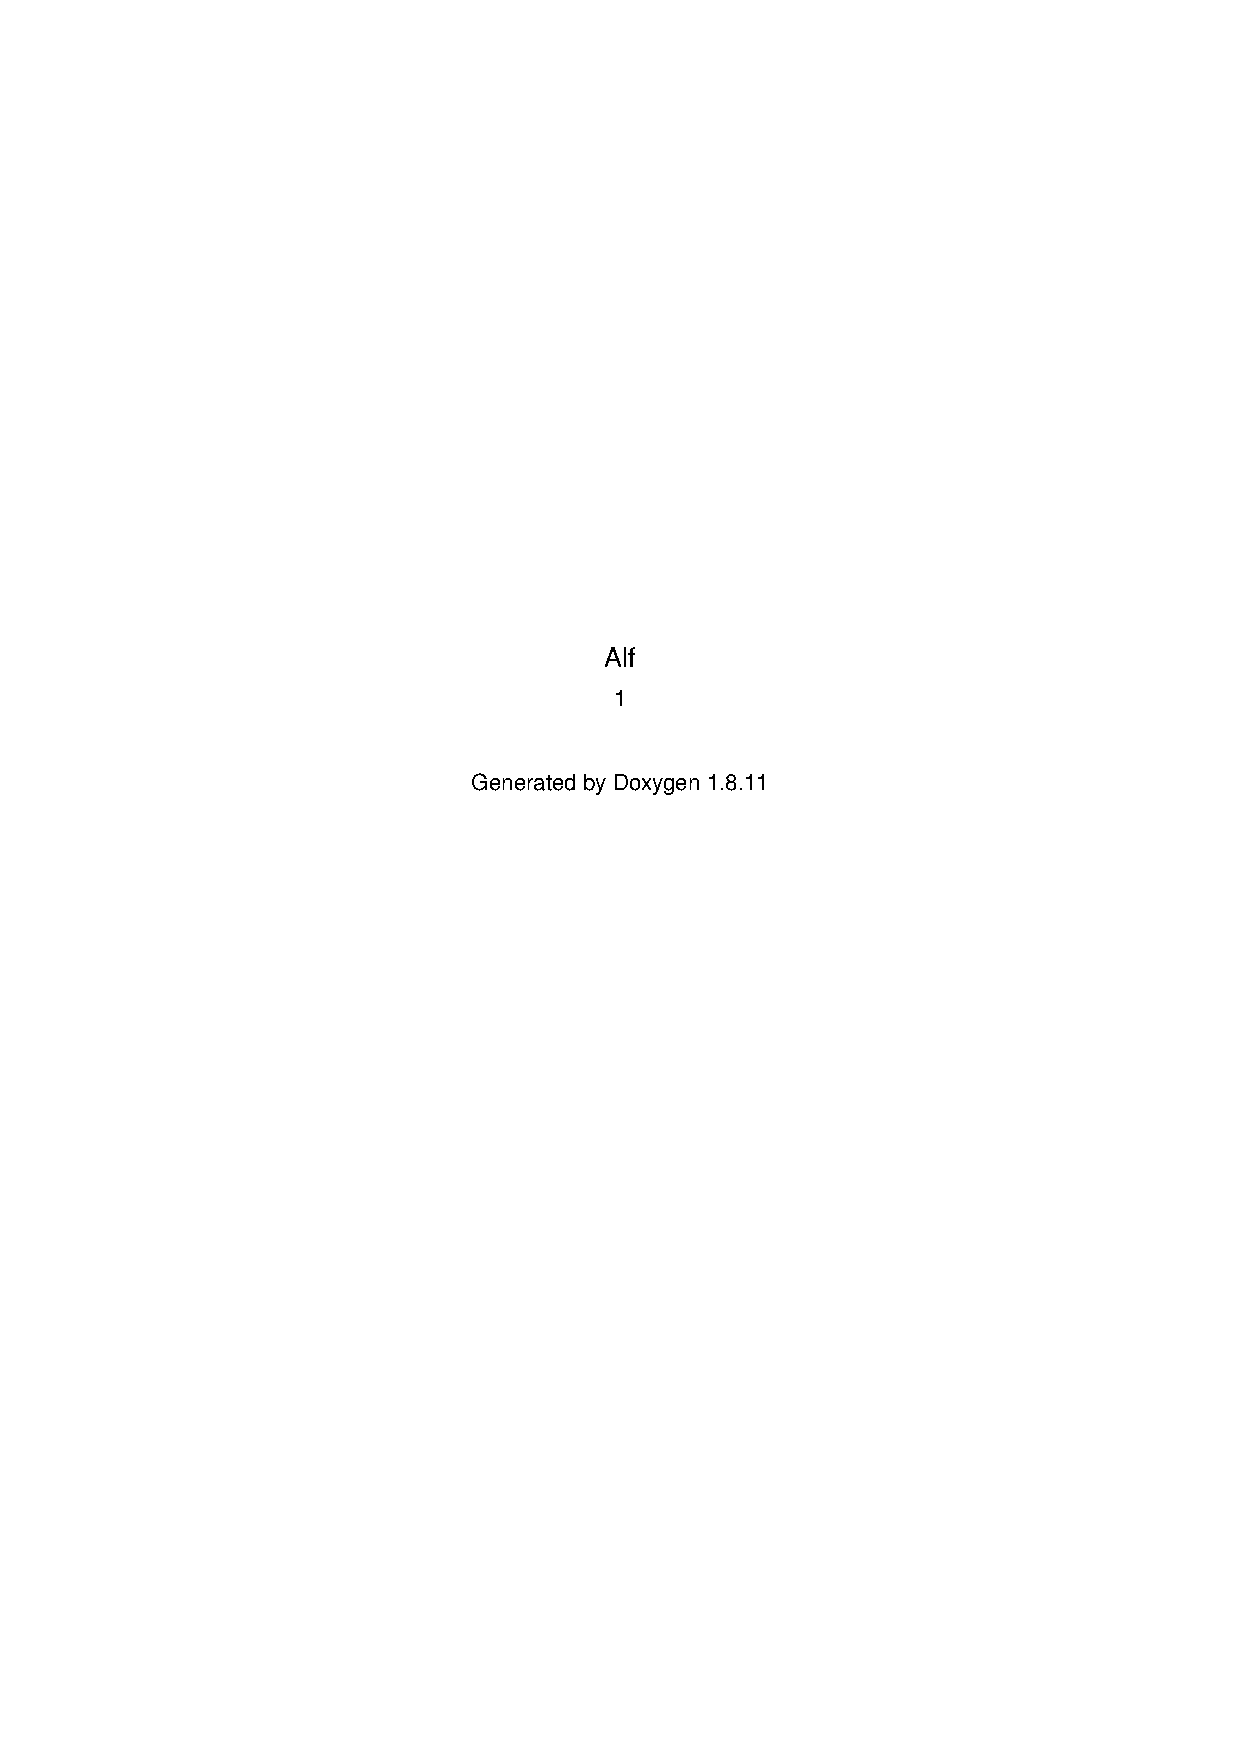
\includepdf[pages=-]{refman.pdf}

\end{document}
